\documentclass[11pt]{article}
\usepackage[textwidth=18.0cm, textheight=23.0cm, top=2.0cm]{geometry}
\usepackage{pst-all}
\usepackage{amssymb}
\usepackage{tikz}
\usepackage{underscore}\begin{document}
\pagestyle{empty}


ClassName: \underline{\textbf{Class_07.2bp-25}}
\par
BinSize: \underline{\textbf{100 × 100}}
\par
ReduceSize: \underline{\textbf{100 × 100}}
\par
TypeNum: \underline{\textbf{60}}
\par
Num: \underline{\textbf{60}}
\par
OutS: \underline{\textbf{150000}}
\par
InS: \underline{\textbf{121269}}
\par
Rate: \underline{\textbf{0.808}}
\par
UB: \underline{\textbf{15}}
\par
LB0: \underline{\textbf{15}}
\par
LB: \underline{\textbf{15}}
\par
LBWithCut: \underline{\textbf{15}}
\par
NodeCut: \underline{\textbf{0}}
\par
ExtendedNodeCnt: \underline{\textbf{1}}
\par
GenNodeCnt: \underline{\textbf{1}}
\par
PrimalNode: \underline{\textbf{0}}
\par
ColumnCount: \underline{\textbf{15}}
\par
TotalCutCount: \underline{\textbf{0}}
\par
RootCutCount: \underline{\textbf{0}}
\par
LPSolverCnt: \underline{\textbf{1}}
\par
PricingSolverCnt: \underline{\textbf{0}}
\par
BranchAndBoundNum: \underline{\textbf{1}}
\par
isOpt: \underline{\textbf{true}}
\par
TimeOnInitSolution: \underline{\textbf{0.020 s}}
\par
TimeOnPrimal: \underline{\textbf{0.000 s}}
\par
TimeOnPricing: \underline{\textbf{0.000 s}}
\par
TimeOnRmp: \underline{\textbf{0.063 s}}
\par
TotalTime: \underline{\textbf{0.145 s}}
\par
\newpage


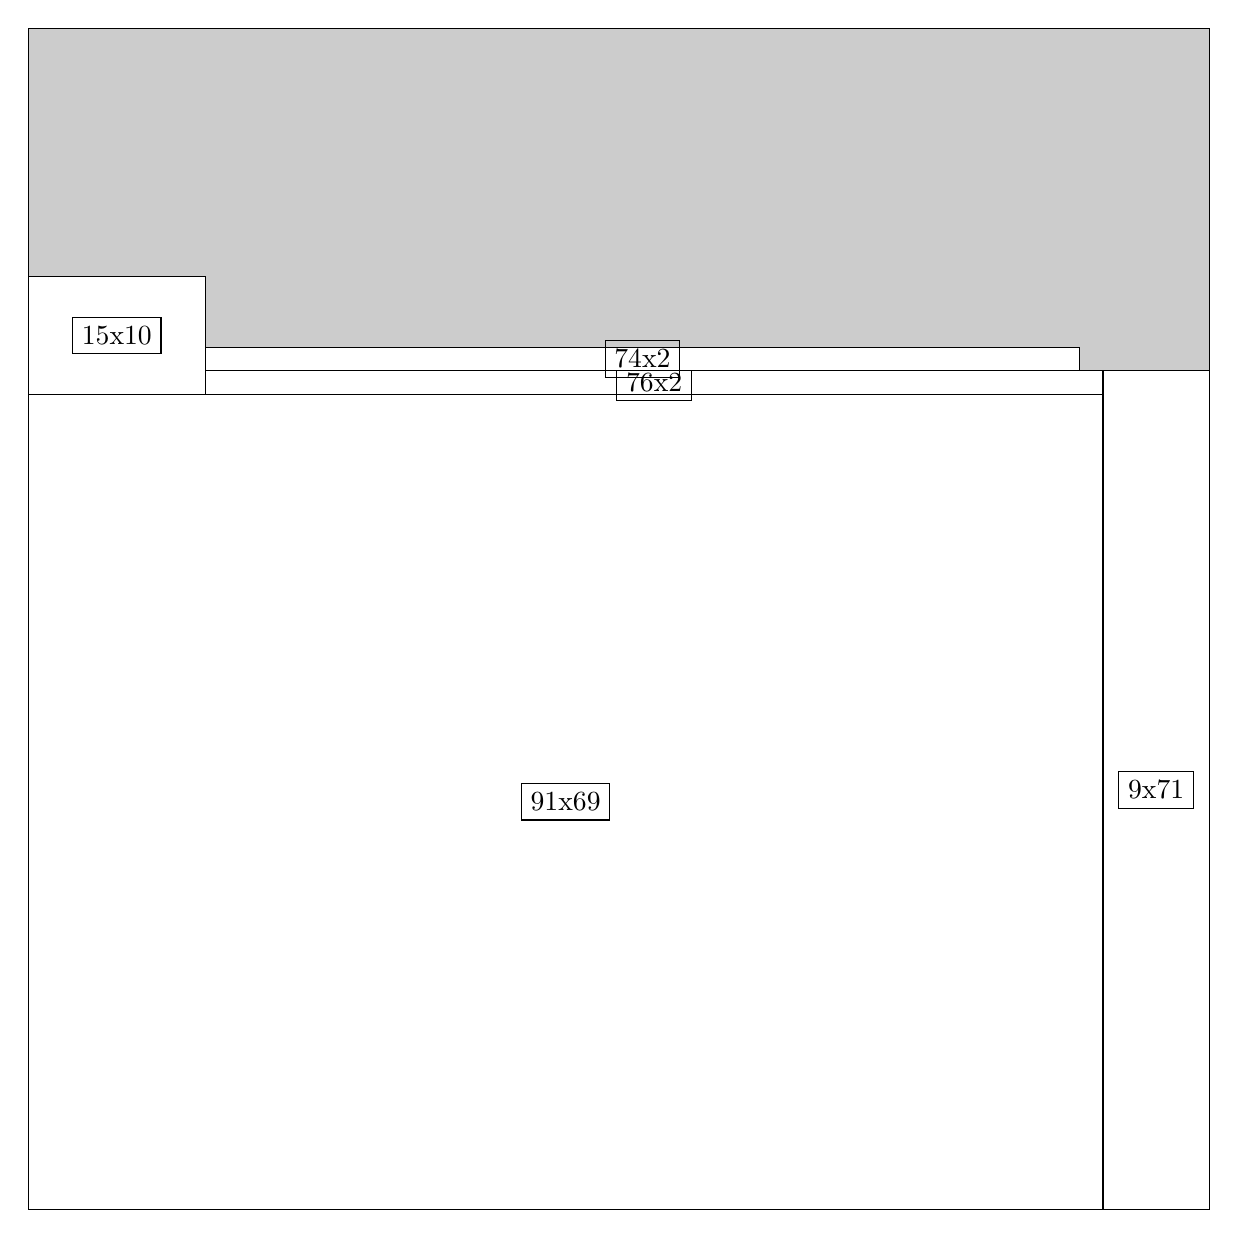
\begin{tikzpicture}[shorten >=1pt,scale=1.0,every node/.style={scale=1.0},->]
\tikzstyle{vertex}=[circle,fill=black!25,minimum size=14pt,inner sep=0pt]
\filldraw[fill=gray!40!white, draw=black] (0,0) rectangle (15.0,15.0);
\foreach \name/\x/\y/\w/\h in {91x69/0.0/0.0/13.65/10.35,9x71/13.65/0.0/1.3499999999999999/10.65,76x2/2.25/10.35/11.4/0.3,15x10/0.0/10.35/2.25/1.5,74x2/2.25/10.65/11.1/0.3}
\filldraw[fill=white!40!white, draw=black] (\x,\y) rectangle node[draw] (\name) {\name} ++(\w,\h);
\end{tikzpicture}


w =91 , h =69 , x =0 , y =0 , v =6279
\par
w =9 , h =71 , x =91 , y =0 , v =639
\par
w =76 , h =2 , x =15 , y =69 , v =152
\par
w =15 , h =10 , x =0 , y =69 , v =150
\par
w =74 , h =2 , x =15 , y =71 , v =148
\par
\newpage


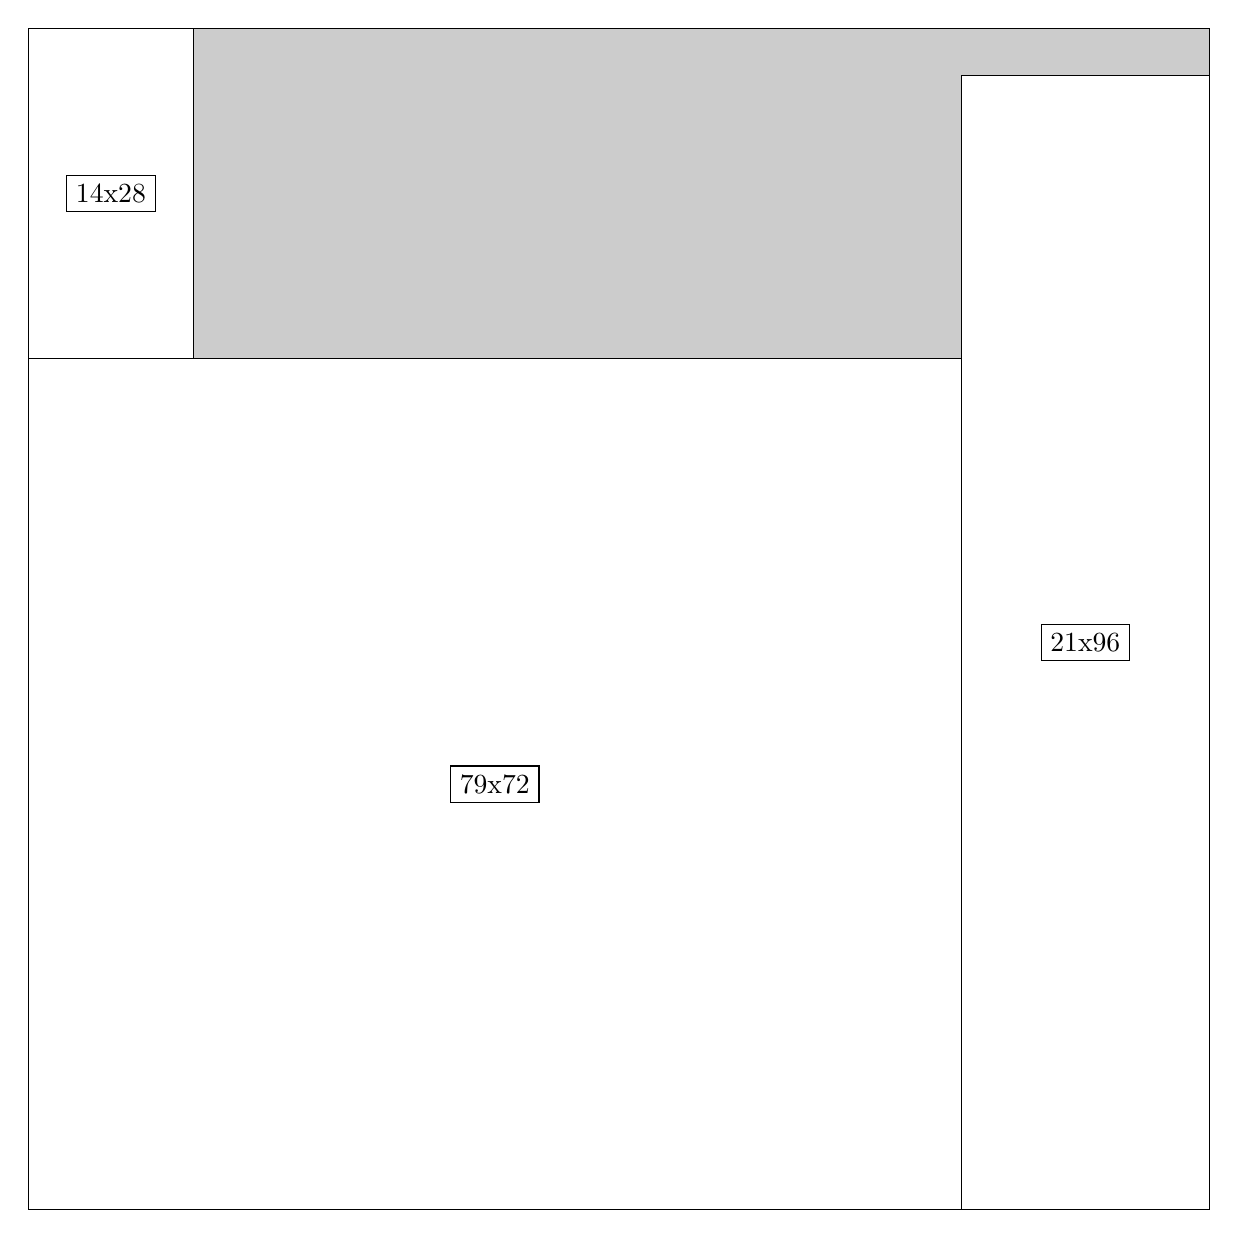
\begin{tikzpicture}[shorten >=1pt,scale=1.0,every node/.style={scale=1.0},->]
\tikzstyle{vertex}=[circle,fill=black!25,minimum size=14pt,inner sep=0pt]
\filldraw[fill=gray!40!white, draw=black] (0,0) rectangle (15.0,15.0);
\foreach \name/\x/\y/\w/\h in {79x72/0.0/0.0/11.85/10.799999999999999,21x96/11.85/0.0/3.15/14.399999999999999,14x28/0.0/10.799999999999999/2.1/4.2}
\filldraw[fill=white!40!white, draw=black] (\x,\y) rectangle node[draw] (\name) {\name} ++(\w,\h);
\end{tikzpicture}


w =79 , h =72 , x =0 , y =0 , v =5688
\par
w =21 , h =96 , x =79 , y =0 , v =2016
\par
w =14 , h =28 , x =0 , y =72 , v =392
\par
\newpage


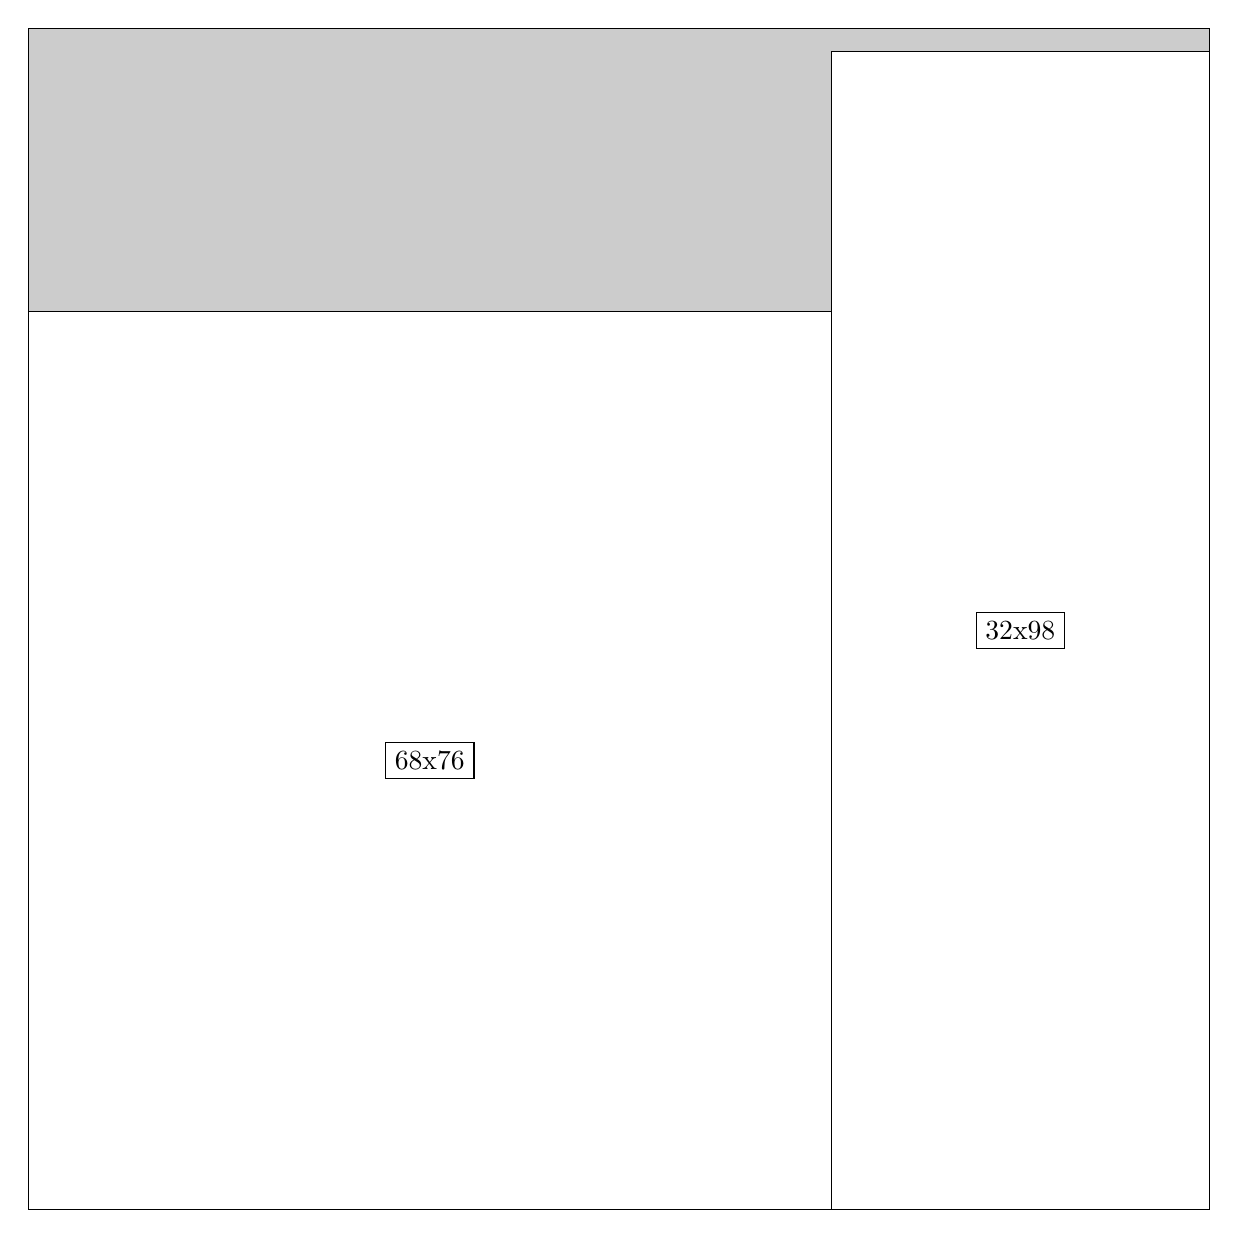
\begin{tikzpicture}[shorten >=1pt,scale=1.0,every node/.style={scale=1.0},->]
\tikzstyle{vertex}=[circle,fill=black!25,minimum size=14pt,inner sep=0pt]
\filldraw[fill=gray!40!white, draw=black] (0,0) rectangle (15.0,15.0);
\foreach \name/\x/\y/\w/\h in {68x76/0.0/0.0/10.2/11.4,32x98/10.2/0.0/4.8/14.7}
\filldraw[fill=white!40!white, draw=black] (\x,\y) rectangle node[draw] (\name) {\name} ++(\w,\h);
\end{tikzpicture}


w =68 , h =76 , x =0 , y =0 , v =5168
\par
w =32 , h =98 , x =68 , y =0 , v =3136
\par
\newpage


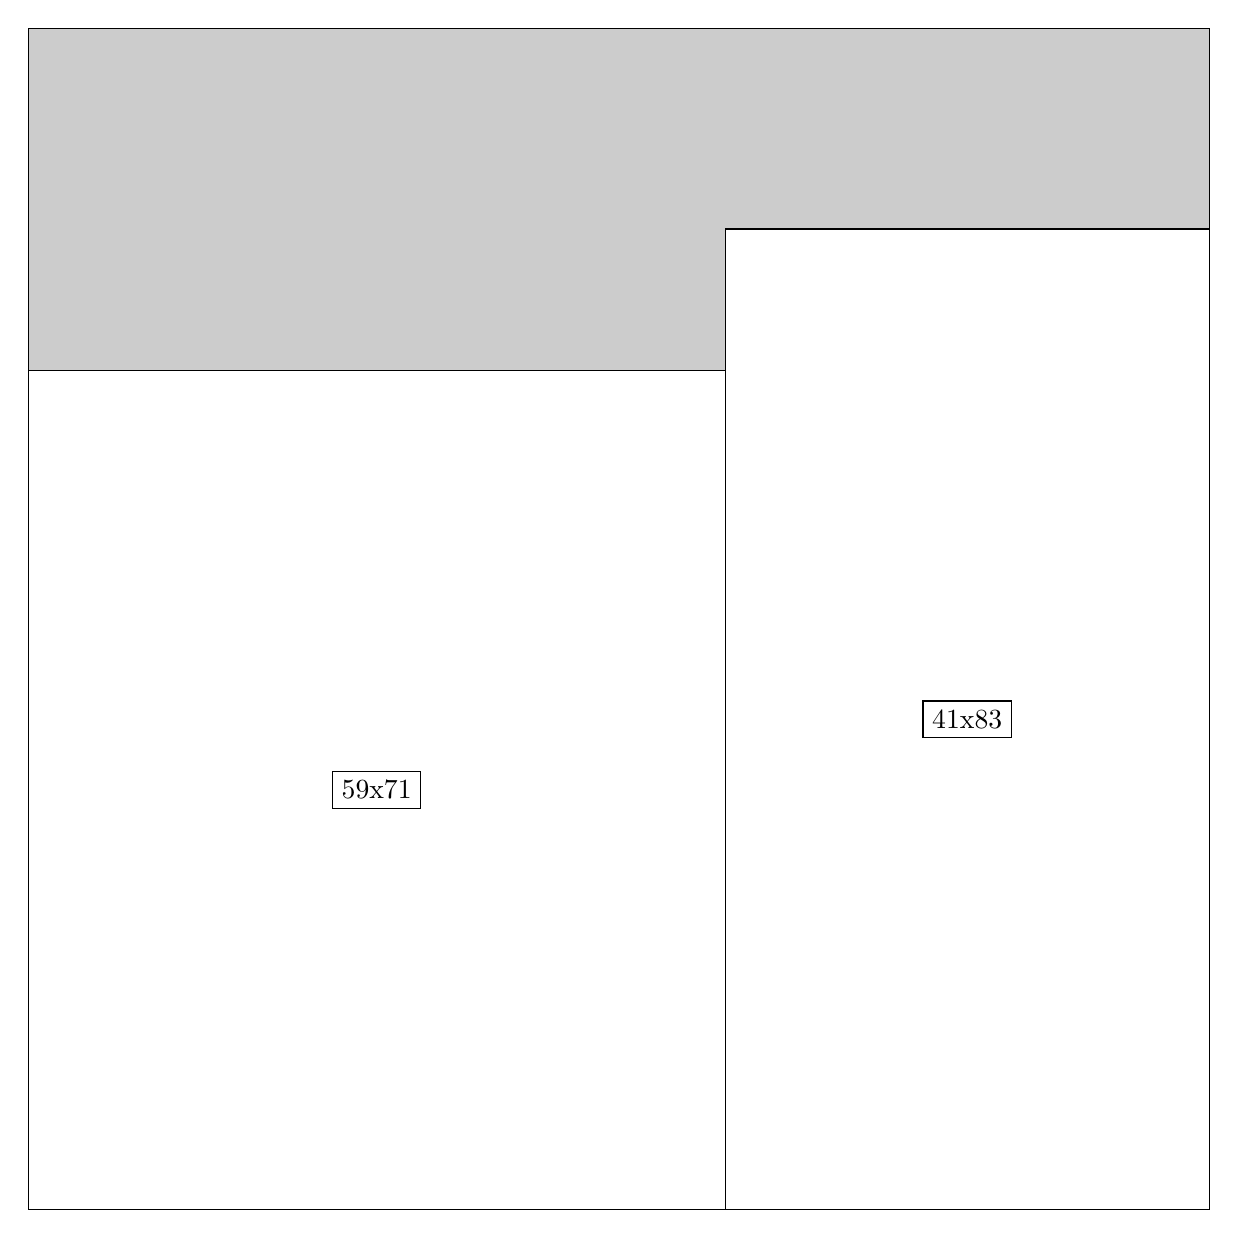
\begin{tikzpicture}[shorten >=1pt,scale=1.0,every node/.style={scale=1.0},->]
\tikzstyle{vertex}=[circle,fill=black!25,minimum size=14pt,inner sep=0pt]
\filldraw[fill=gray!40!white, draw=black] (0,0) rectangle (15.0,15.0);
\foreach \name/\x/\y/\w/\h in {59x71/0.0/0.0/8.85/10.65,41x83/8.85/0.0/6.1499999999999995/12.45}
\filldraw[fill=white!40!white, draw=black] (\x,\y) rectangle node[draw] (\name) {\name} ++(\w,\h);
\end{tikzpicture}


w =59 , h =71 , x =0 , y =0 , v =4189
\par
w =41 , h =83 , x =59 , y =0 , v =3403
\par
\newpage


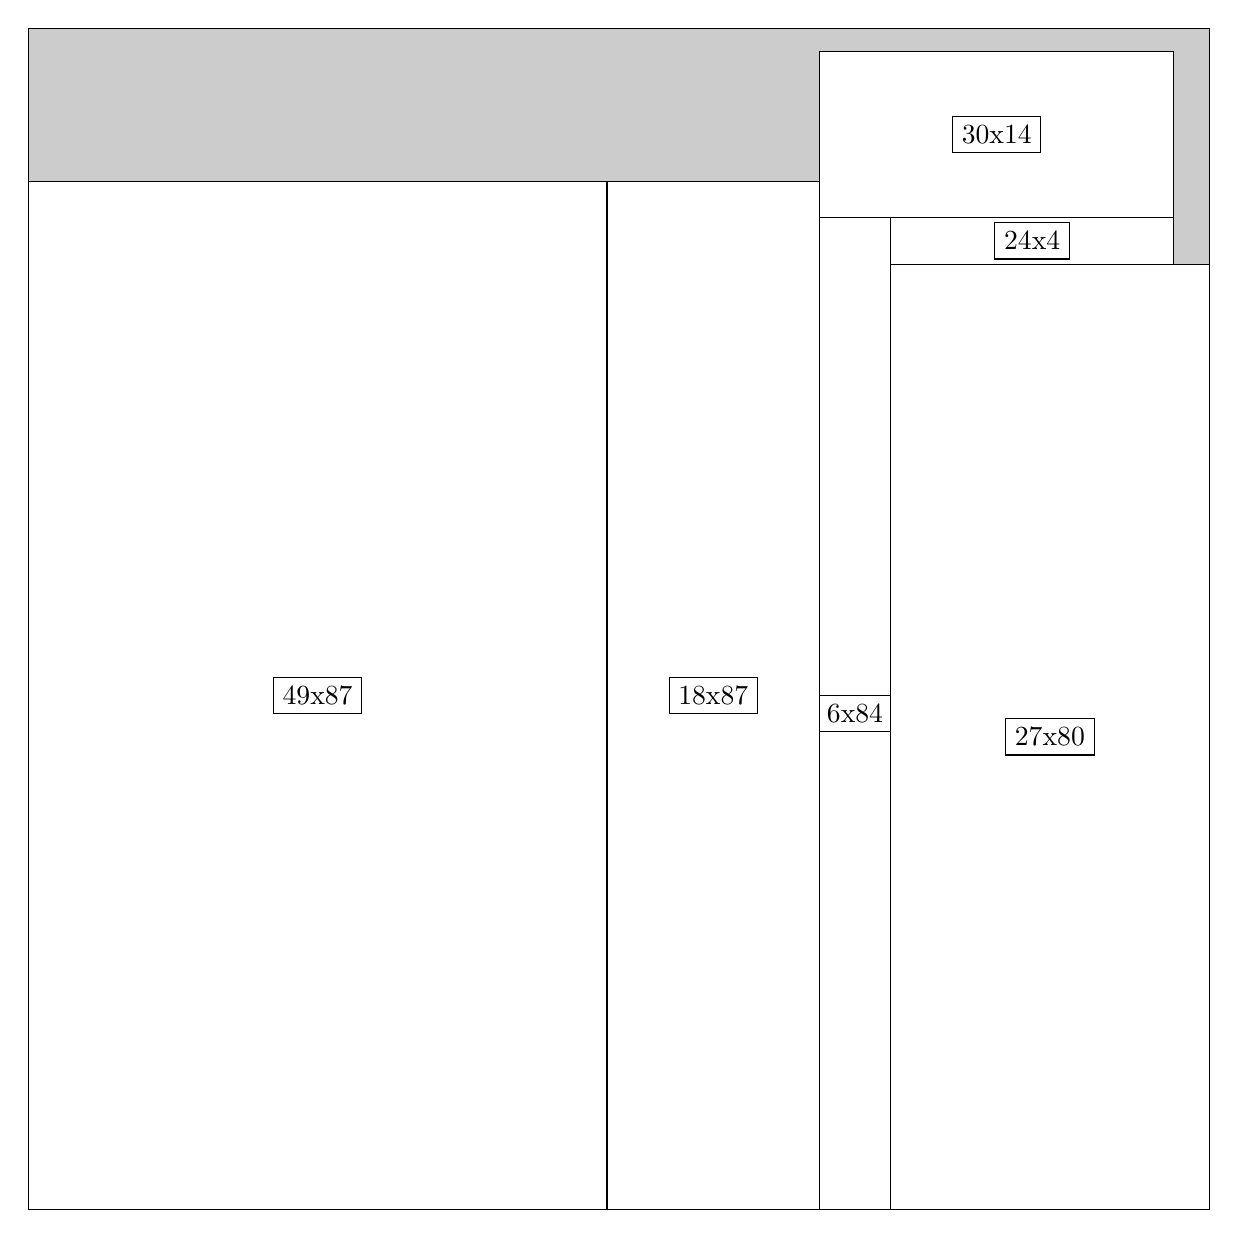
\begin{tikzpicture}[shorten >=1pt,scale=1.0,every node/.style={scale=1.0},->]
\tikzstyle{vertex}=[circle,fill=black!25,minimum size=14pt,inner sep=0pt]
\filldraw[fill=gray!40!white, draw=black] (0,0) rectangle (15.0,15.0);
\foreach \name/\x/\y/\w/\h in {49x87/0.0/0.0/7.35/13.049999999999999,6x84/10.049999999999999/0.0/0.8999999999999999/12.6,27x80/10.95/0.0/4.05/12.0,18x87/7.35/0.0/2.6999999999999997/13.049999999999999,30x14/10.049999999999999/12.6/4.5/2.1,24x4/10.95/12.0/3.5999999999999996/0.6}
\filldraw[fill=white!40!white, draw=black] (\x,\y) rectangle node[draw] (\name) {\name} ++(\w,\h);
\end{tikzpicture}


w =49 , h =87 , x =0 , y =0 , v =4263
\par
w =6 , h =84 , x =67 , y =0 , v =504
\par
w =27 , h =80 , x =73 , y =0 , v =2160
\par
w =18 , h =87 , x =49 , y =0 , v =1566
\par
w =30 , h =14 , x =67 , y =84 , v =420
\par
w =24 , h =4 , x =73 , y =80 , v =96
\par
\newpage


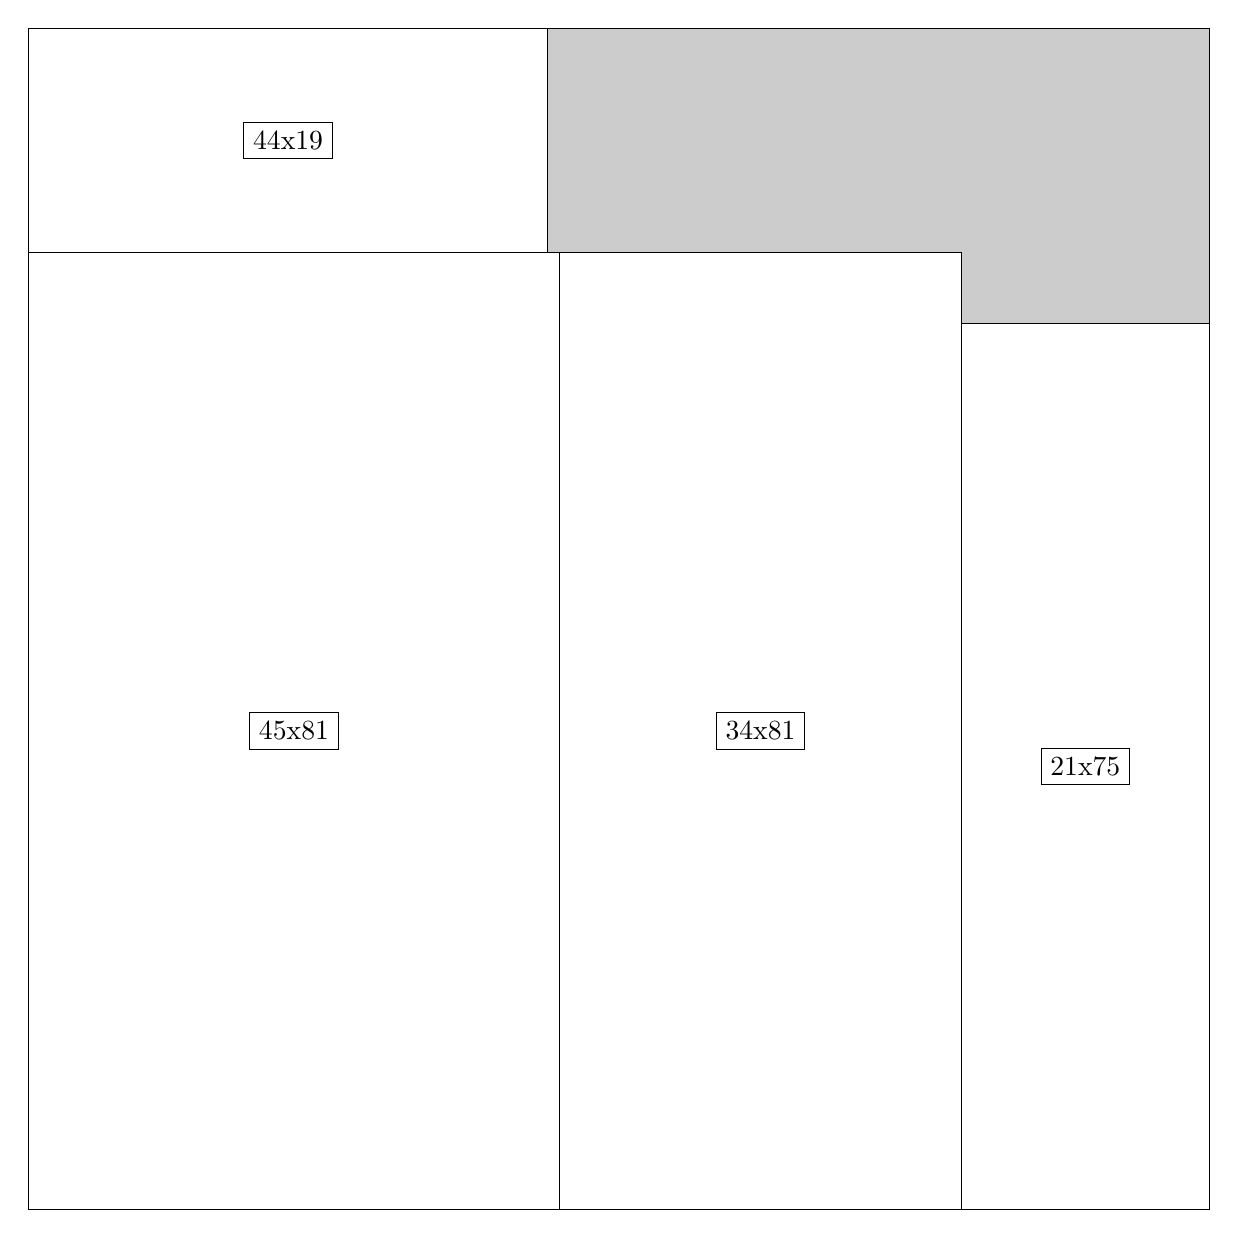
\begin{tikzpicture}[shorten >=1pt,scale=1.0,every node/.style={scale=1.0},->]
\tikzstyle{vertex}=[circle,fill=black!25,minimum size=14pt,inner sep=0pt]
\filldraw[fill=gray!40!white, draw=black] (0,0) rectangle (15.0,15.0);
\foreach \name/\x/\y/\w/\h in {45x81/0.0/0.0/6.75/12.15,34x81/6.75/0.0/5.1/12.15,21x75/11.85/0.0/3.15/11.25,44x19/0.0/12.15/6.6/2.85}
\filldraw[fill=white!40!white, draw=black] (\x,\y) rectangle node[draw] (\name) {\name} ++(\w,\h);
\end{tikzpicture}


w =45 , h =81 , x =0 , y =0 , v =3645
\par
w =34 , h =81 , x =45 , y =0 , v =2754
\par
w =21 , h =75 , x =79 , y =0 , v =1575
\par
w =44 , h =19 , x =0 , y =81 , v =836
\par
\newpage


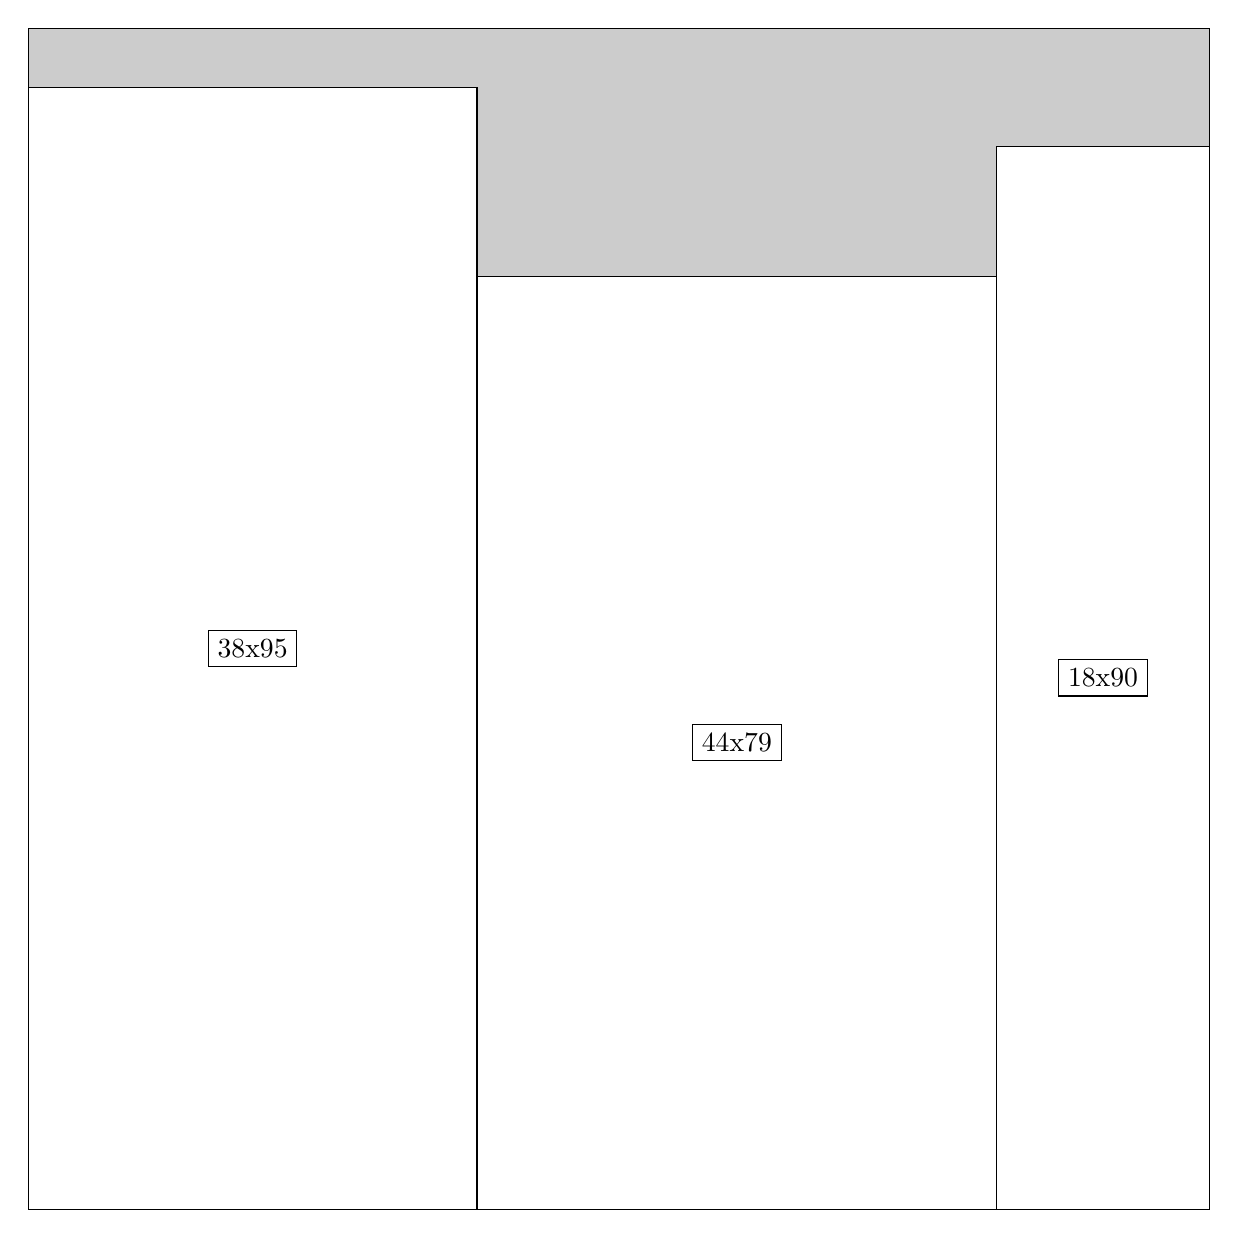
\begin{tikzpicture}[shorten >=1pt,scale=1.0,every node/.style={scale=1.0},->]
\tikzstyle{vertex}=[circle,fill=black!25,minimum size=14pt,inner sep=0pt]
\filldraw[fill=gray!40!white, draw=black] (0,0) rectangle (15.0,15.0);
\foreach \name/\x/\y/\w/\h in {38x95/0.0/0.0/5.7/14.25,44x79/5.7/0.0/6.6/11.85,18x90/12.299999999999999/0.0/2.6999999999999997/13.5}
\filldraw[fill=white!40!white, draw=black] (\x,\y) rectangle node[draw] (\name) {\name} ++(\w,\h);
\end{tikzpicture}


w =38 , h =95 , x =0 , y =0 , v =3610
\par
w =44 , h =79 , x =38 , y =0 , v =3476
\par
w =18 , h =90 , x =82 , y =0 , v =1620
\par
\newpage


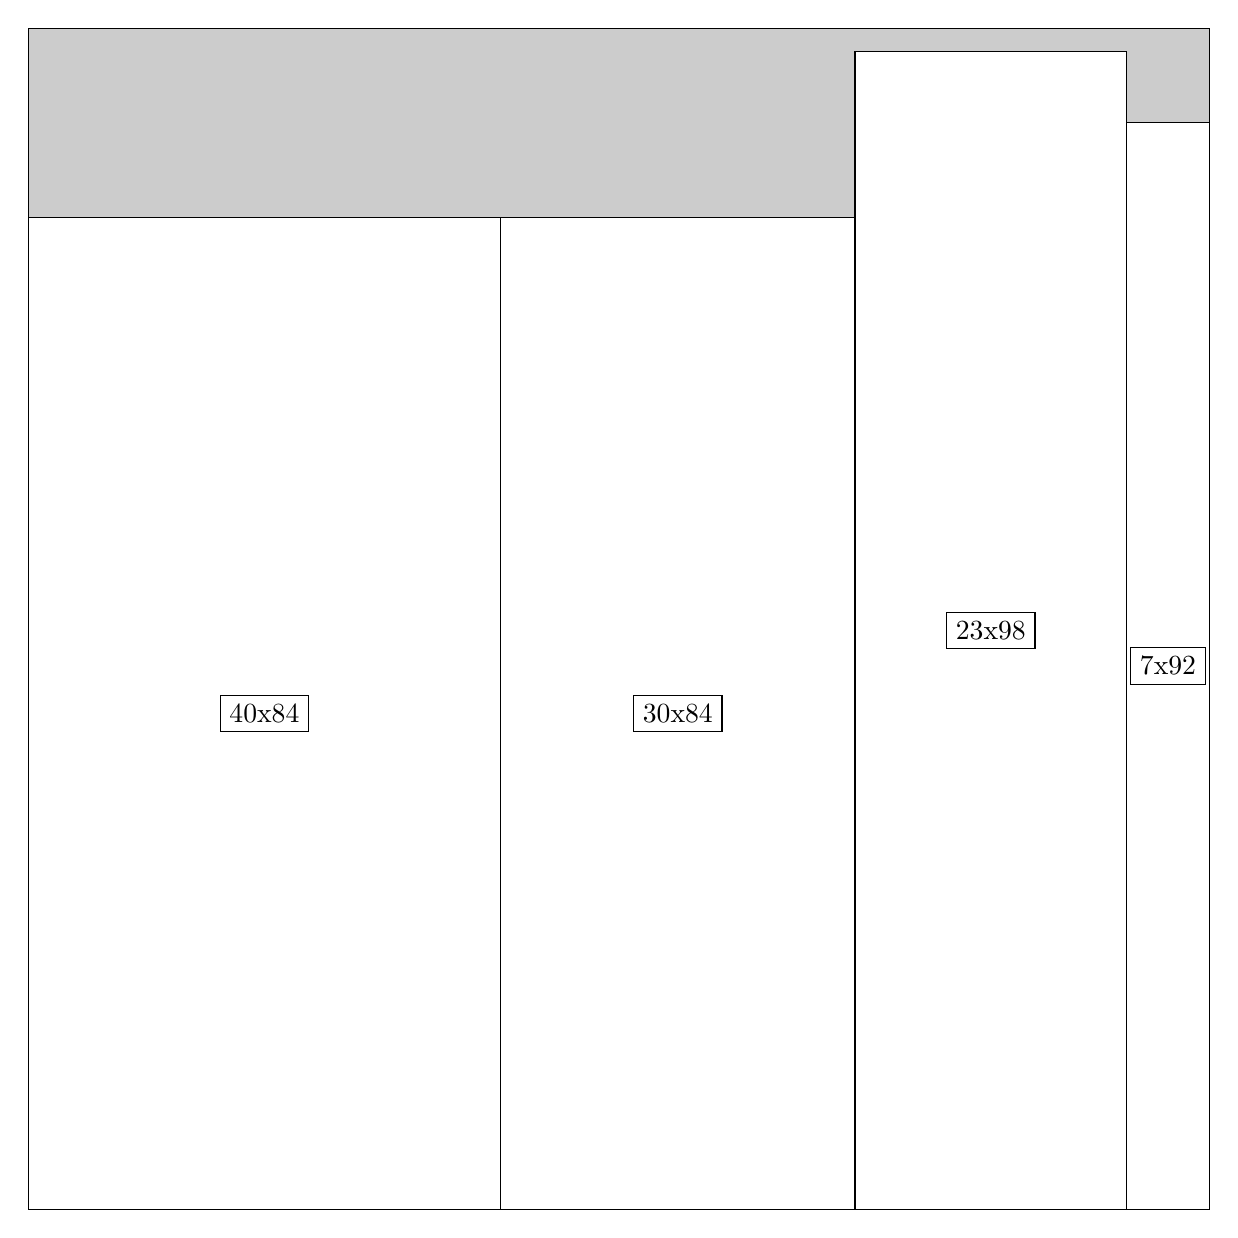
\begin{tikzpicture}[shorten >=1pt,scale=1.0,every node/.style={scale=1.0},->]
\tikzstyle{vertex}=[circle,fill=black!25,minimum size=14pt,inner sep=0pt]
\filldraw[fill=gray!40!white, draw=black] (0,0) rectangle (15.0,15.0);
\foreach \name/\x/\y/\w/\h in {40x84/0.0/0.0/6.0/12.6,30x84/6.0/0.0/4.5/12.6,23x98/10.5/0.0/3.4499999999999997/14.7,7x92/13.95/0.0/1.05/13.799999999999999}
\filldraw[fill=white!40!white, draw=black] (\x,\y) rectangle node[draw] (\name) {\name} ++(\w,\h);
\end{tikzpicture}


w =40 , h =84 , x =0 , y =0 , v =3360
\par
w =30 , h =84 , x =40 , y =0 , v =2520
\par
w =23 , h =98 , x =70 , y =0 , v =2254
\par
w =7 , h =92 , x =93 , y =0 , v =644
\par
\newpage


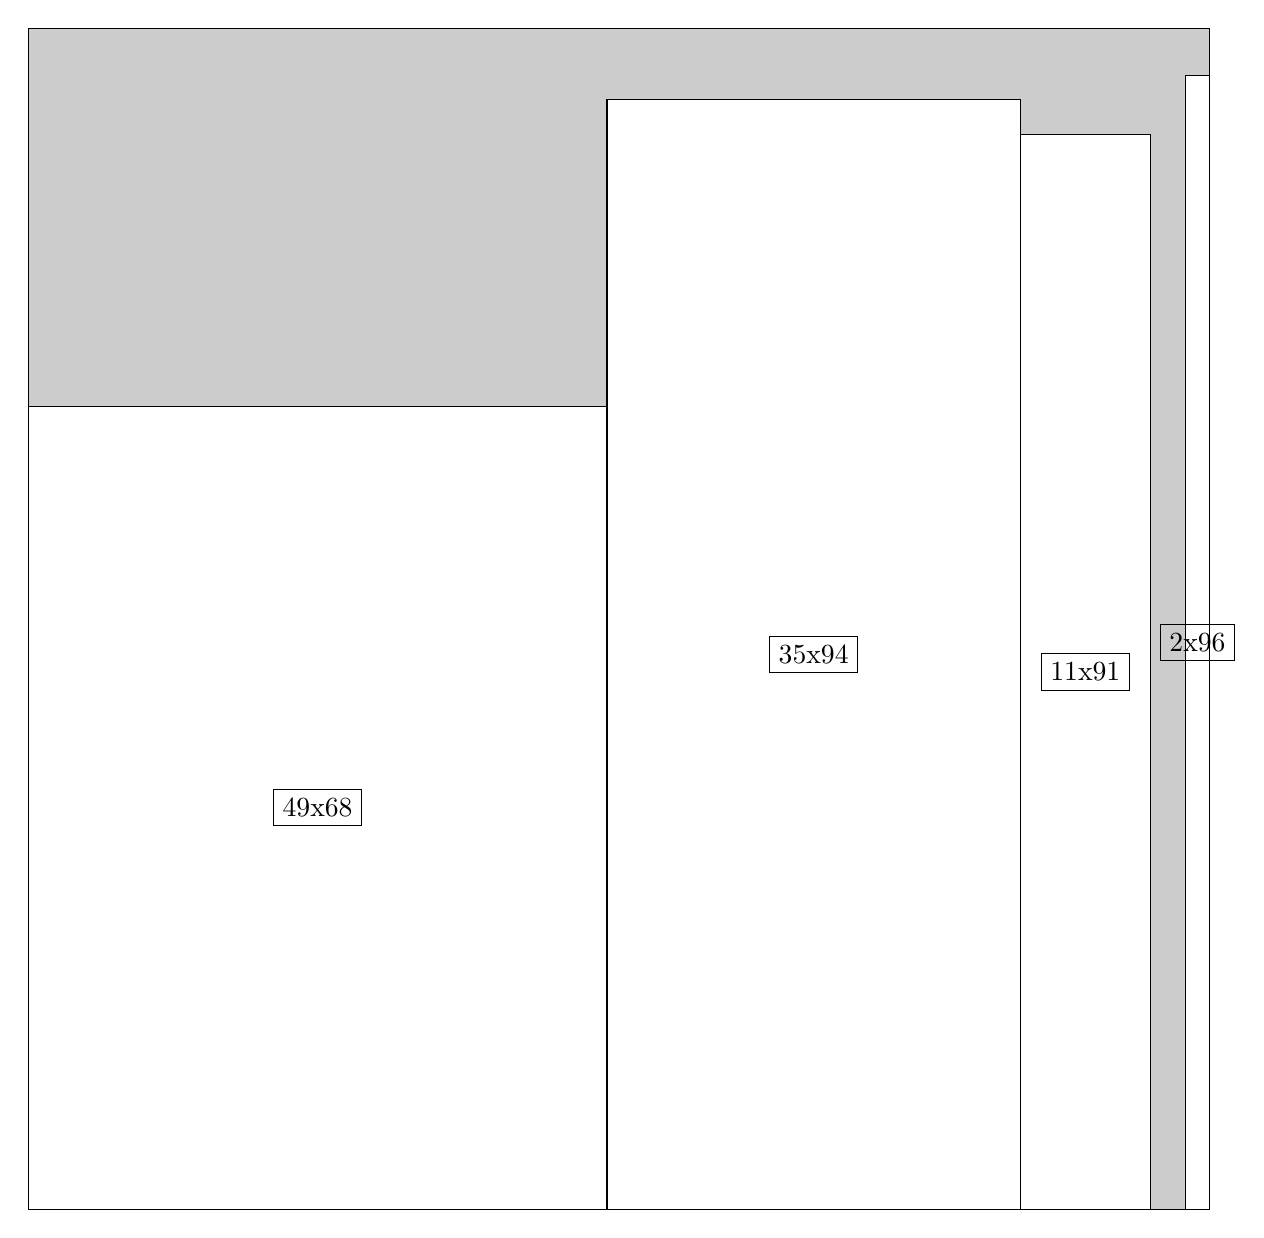
\begin{tikzpicture}[shorten >=1pt,scale=1.0,every node/.style={scale=1.0},->]
\tikzstyle{vertex}=[circle,fill=black!25,minimum size=14pt,inner sep=0pt]
\filldraw[fill=gray!40!white, draw=black] (0,0) rectangle (15.0,15.0);
\foreach \name/\x/\y/\w/\h in {49x68/0.0/0.0/7.35/10.2,35x94/7.35/0.0/5.25/14.1,11x91/12.6/0.0/1.65/13.65,2x96/14.7/0.0/0.3/14.399999999999999}
\filldraw[fill=white!40!white, draw=black] (\x,\y) rectangle node[draw] (\name) {\name} ++(\w,\h);
\end{tikzpicture}


w =49 , h =68 , x =0 , y =0 , v =3332
\par
w =35 , h =94 , x =49 , y =0 , v =3290
\par
w =11 , h =91 , x =84 , y =0 , v =1001
\par
w =2 , h =96 , x =98 , y =0 , v =192
\par
\newpage


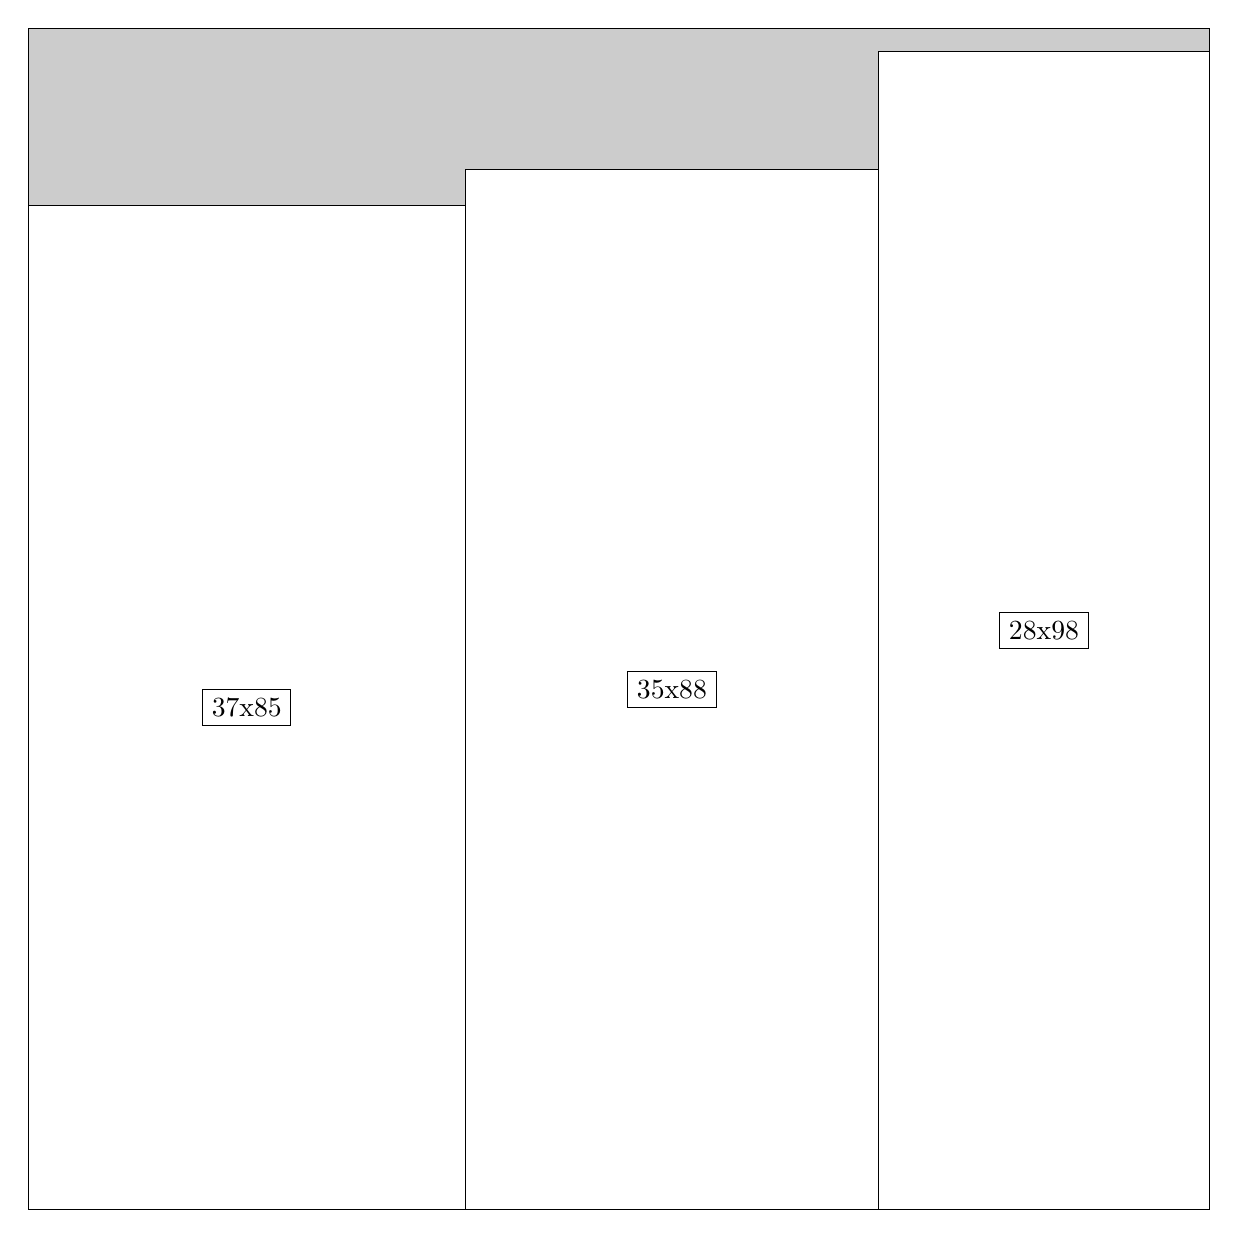
\begin{tikzpicture}[shorten >=1pt,scale=1.0,every node/.style={scale=1.0},->]
\tikzstyle{vertex}=[circle,fill=black!25,minimum size=14pt,inner sep=0pt]
\filldraw[fill=gray!40!white, draw=black] (0,0) rectangle (15.0,15.0);
\foreach \name/\x/\y/\w/\h in {37x85/0.0/0.0/5.55/12.75,35x88/5.55/0.0/5.25/13.2,28x98/10.799999999999999/0.0/4.2/14.7}
\filldraw[fill=white!40!white, draw=black] (\x,\y) rectangle node[draw] (\name) {\name} ++(\w,\h);
\end{tikzpicture}


w =37 , h =85 , x =0 , y =0 , v =3145
\par
w =35 , h =88 , x =37 , y =0 , v =3080
\par
w =28 , h =98 , x =72 , y =0 , v =2744
\par
\newpage


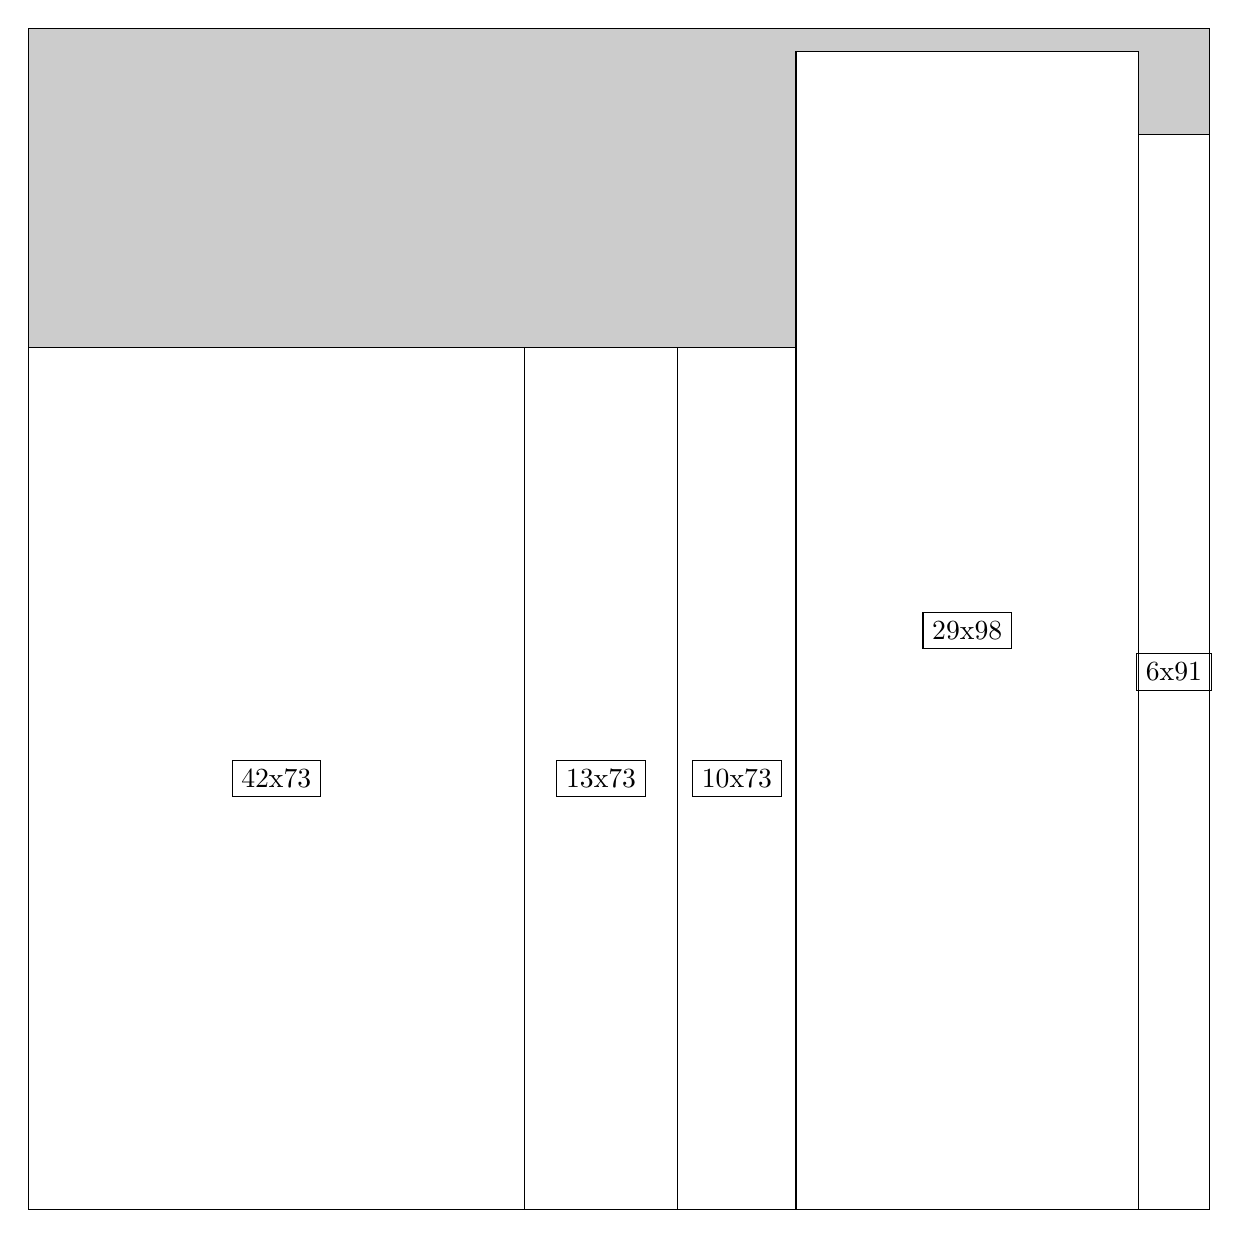
\begin{tikzpicture}[shorten >=1pt,scale=1.0,every node/.style={scale=1.0},->]
\tikzstyle{vertex}=[circle,fill=black!25,minimum size=14pt,inner sep=0pt]
\filldraw[fill=gray!40!white, draw=black] (0,0) rectangle (15.0,15.0);
\foreach \name/\x/\y/\w/\h in {42x73/0.0/0.0/6.3/10.95,29x98/9.75/0.0/4.35/14.7,13x73/6.3/0.0/1.95/10.95,10x73/8.25/0.0/1.5/10.95,6x91/14.1/0.0/0.8999999999999999/13.65}
\filldraw[fill=white!40!white, draw=black] (\x,\y) rectangle node[draw] (\name) {\name} ++(\w,\h);
\end{tikzpicture}


w =42 , h =73 , x =0 , y =0 , v =3066
\par
w =29 , h =98 , x =65 , y =0 , v =2842
\par
w =13 , h =73 , x =42 , y =0 , v =949
\par
w =10 , h =73 , x =55 , y =0 , v =730
\par
w =6 , h =91 , x =94 , y =0 , v =546
\par
\newpage


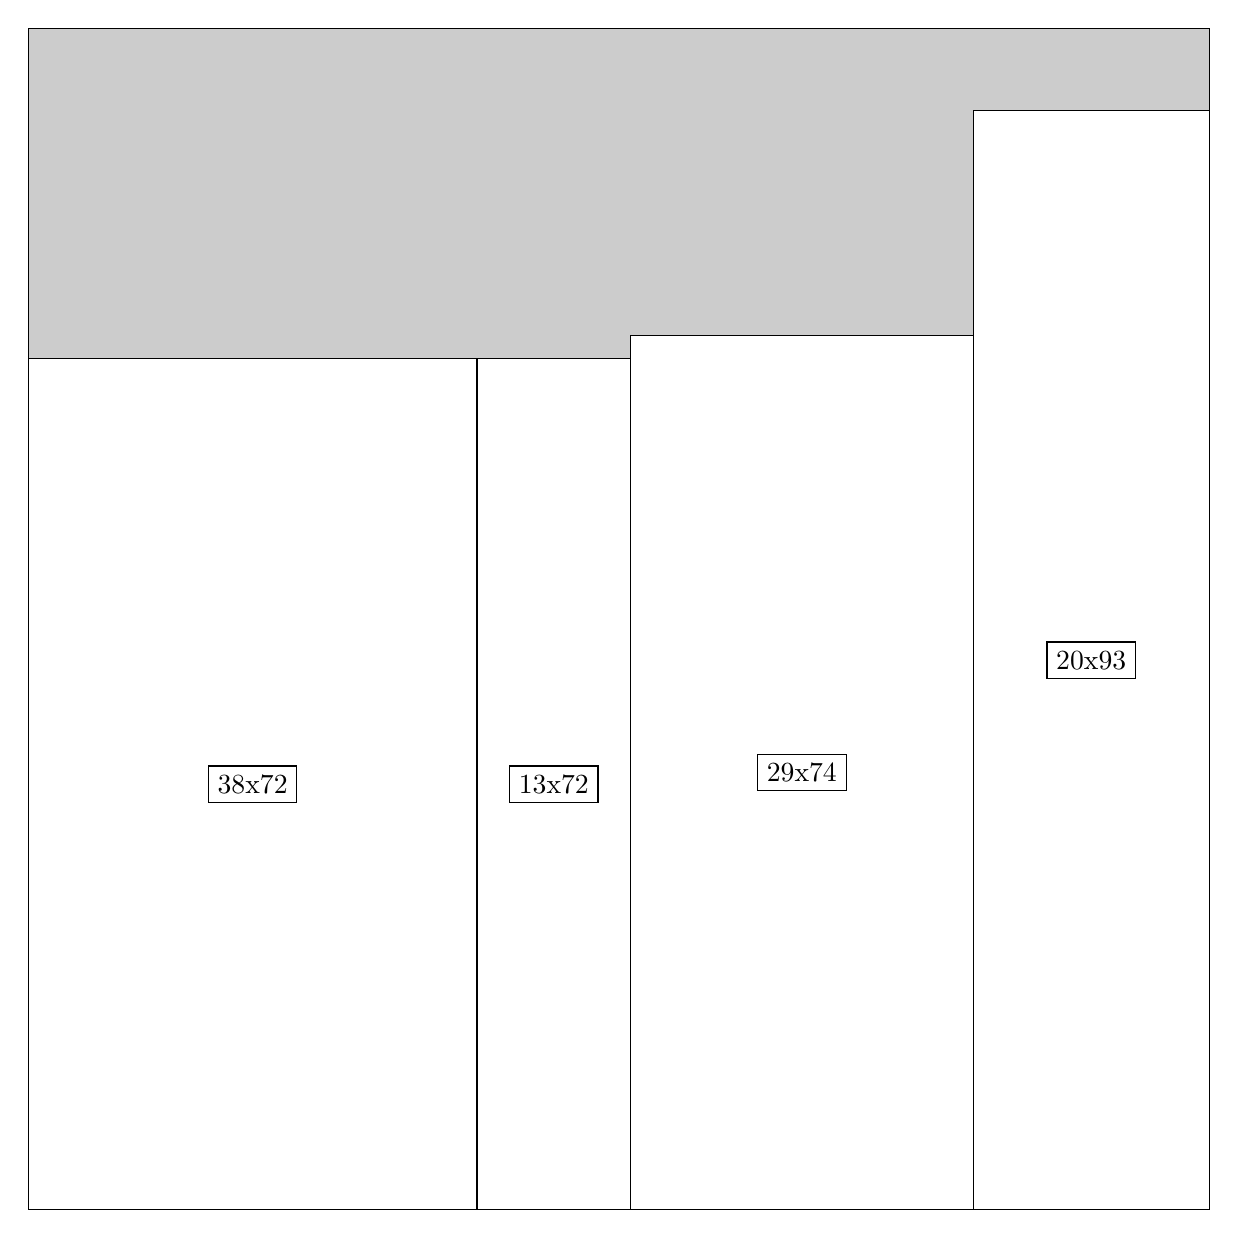
\begin{tikzpicture}[shorten >=1pt,scale=1.0,every node/.style={scale=1.0},->]
\tikzstyle{vertex}=[circle,fill=black!25,minimum size=14pt,inner sep=0pt]
\filldraw[fill=gray!40!white, draw=black] (0,0) rectangle (15.0,15.0);
\foreach \name/\x/\y/\w/\h in {38x72/0.0/0.0/5.7/10.799999999999999,29x74/7.6499999999999995/0.0/4.35/11.1,20x93/12.0/0.0/3.0/13.95,13x72/5.7/0.0/1.95/10.799999999999999}
\filldraw[fill=white!40!white, draw=black] (\x,\y) rectangle node[draw] (\name) {\name} ++(\w,\h);
\end{tikzpicture}


w =38 , h =72 , x =0 , y =0 , v =2736
\par
w =29 , h =74 , x =51 , y =0 , v =2146
\par
w =20 , h =93 , x =80 , y =0 , v =1860
\par
w =13 , h =72 , x =38 , y =0 , v =936
\par
\newpage


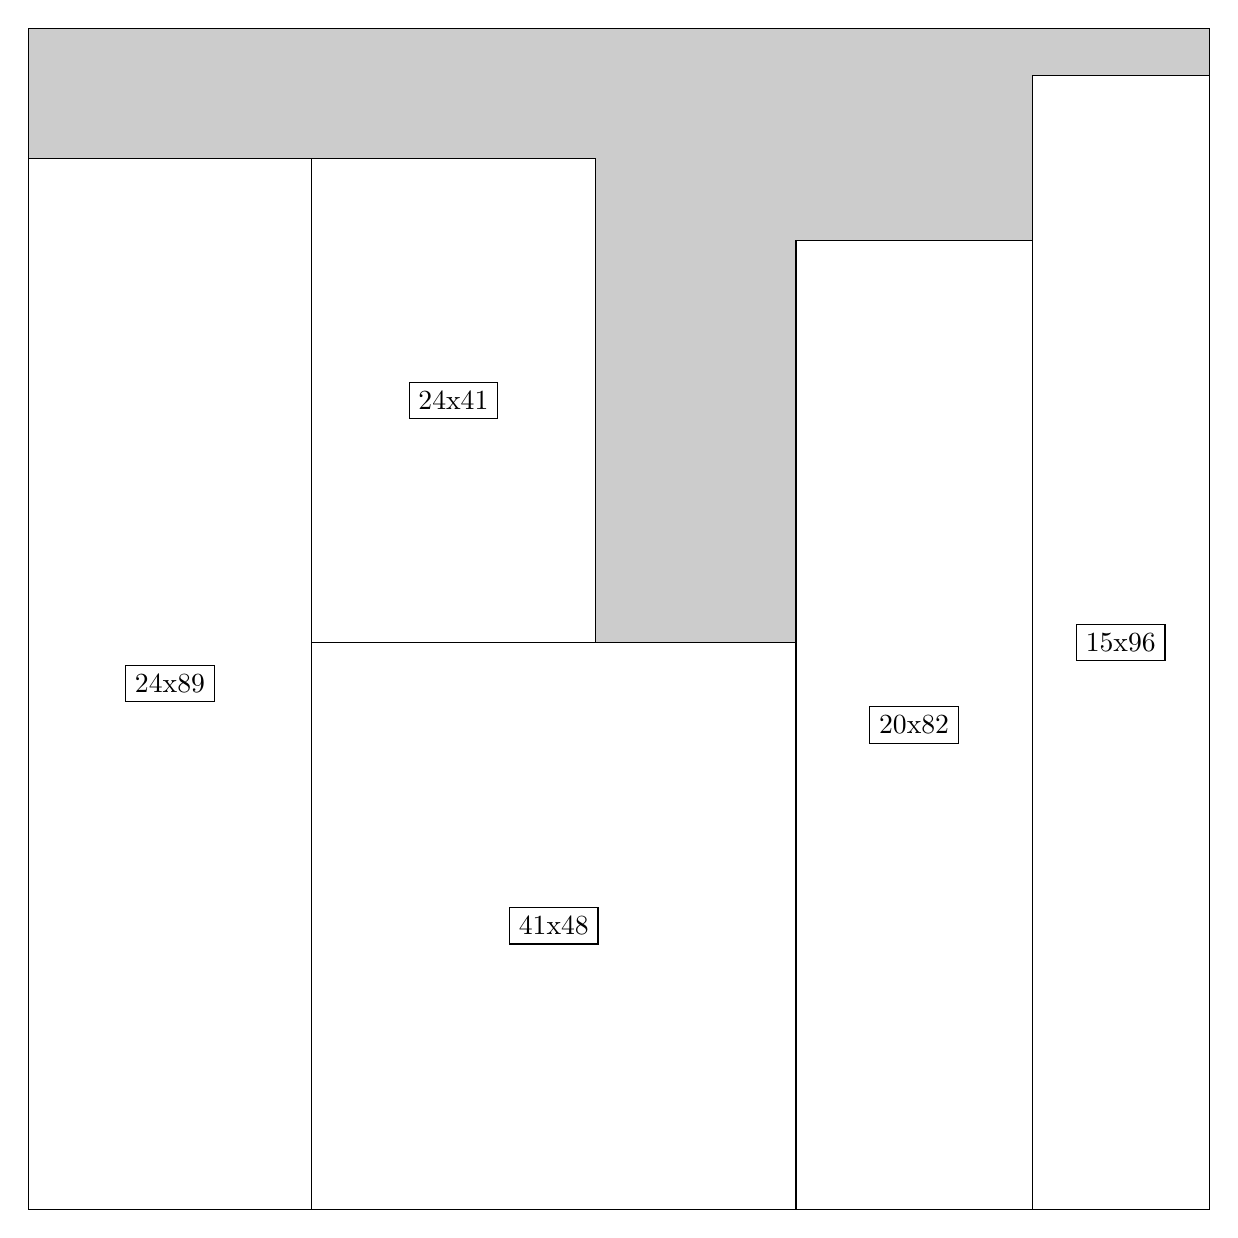
\begin{tikzpicture}[shorten >=1pt,scale=1.0,every node/.style={scale=1.0},->]
\tikzstyle{vertex}=[circle,fill=black!25,minimum size=14pt,inner sep=0pt]
\filldraw[fill=gray!40!white, draw=black] (0,0) rectangle (15.0,15.0);
\foreach \name/\x/\y/\w/\h in {24x89/0.0/0.0/3.5999999999999996/13.35,41x48/3.5999999999999996/0.0/6.1499999999999995/7.199999999999999,20x82/9.75/0.0/3.0/12.299999999999999,15x96/12.75/0.0/2.25/14.399999999999999,24x41/3.5999999999999996/7.199999999999999/3.5999999999999996/6.1499999999999995}
\filldraw[fill=white!40!white, draw=black] (\x,\y) rectangle node[draw] (\name) {\name} ++(\w,\h);
\end{tikzpicture}


w =24 , h =89 , x =0 , y =0 , v =2136
\par
w =41 , h =48 , x =24 , y =0 , v =1968
\par
w =20 , h =82 , x =65 , y =0 , v =1640
\par
w =15 , h =96 , x =85 , y =0 , v =1440
\par
w =24 , h =41 , x =24 , y =48 , v =984
\par
\newpage


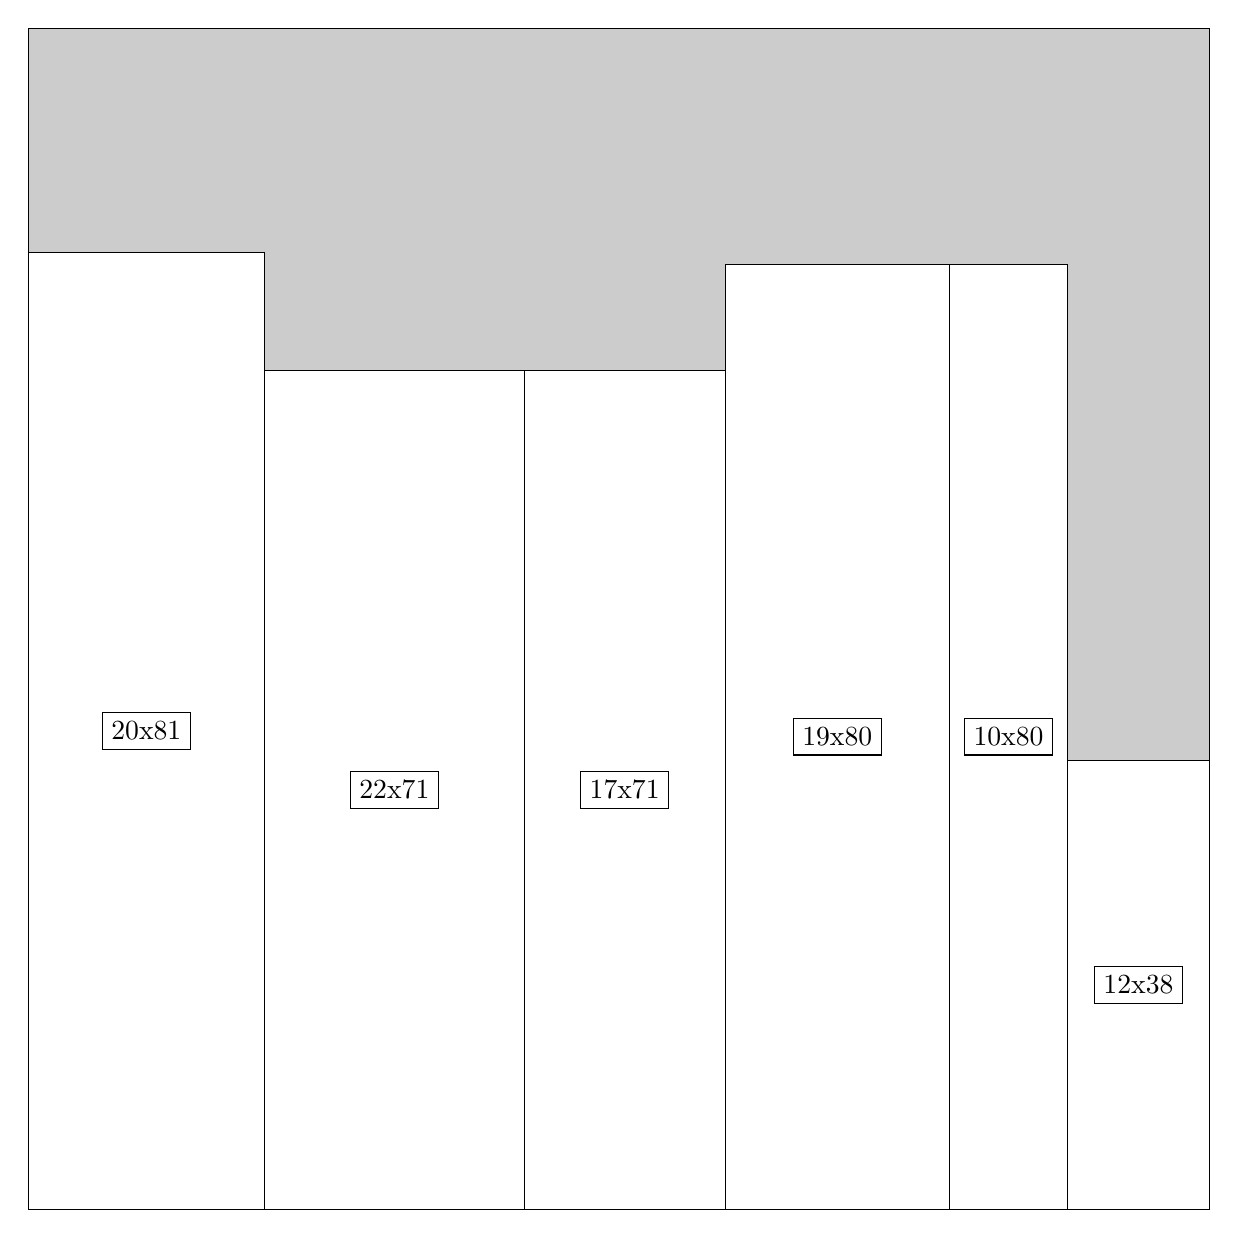
\begin{tikzpicture}[shorten >=1pt,scale=1.0,every node/.style={scale=1.0},->]
\tikzstyle{vertex}=[circle,fill=black!25,minimum size=14pt,inner sep=0pt]
\filldraw[fill=gray!40!white, draw=black] (0,0) rectangle (15.0,15.0);
\foreach \name/\x/\y/\w/\h in {20x81/0.0/0.0/3.0/12.15,22x71/3.0/0.0/3.3/10.65,19x80/8.85/0.0/2.85/12.0,17x71/6.3/0.0/2.55/10.65,10x80/11.7/0.0/1.5/12.0,12x38/13.2/0.0/1.7999999999999998/5.7}
\filldraw[fill=white!40!white, draw=black] (\x,\y) rectangle node[draw] (\name) {\name} ++(\w,\h);
\end{tikzpicture}


w =20 , h =81 , x =0 , y =0 , v =1620
\par
w =22 , h =71 , x =20 , y =0 , v =1562
\par
w =19 , h =80 , x =59 , y =0 , v =1520
\par
w =17 , h =71 , x =42 , y =0 , v =1207
\par
w =10 , h =80 , x =78 , y =0 , v =800
\par
w =12 , h =38 , x =88 , y =0 , v =456
\par
\newpage


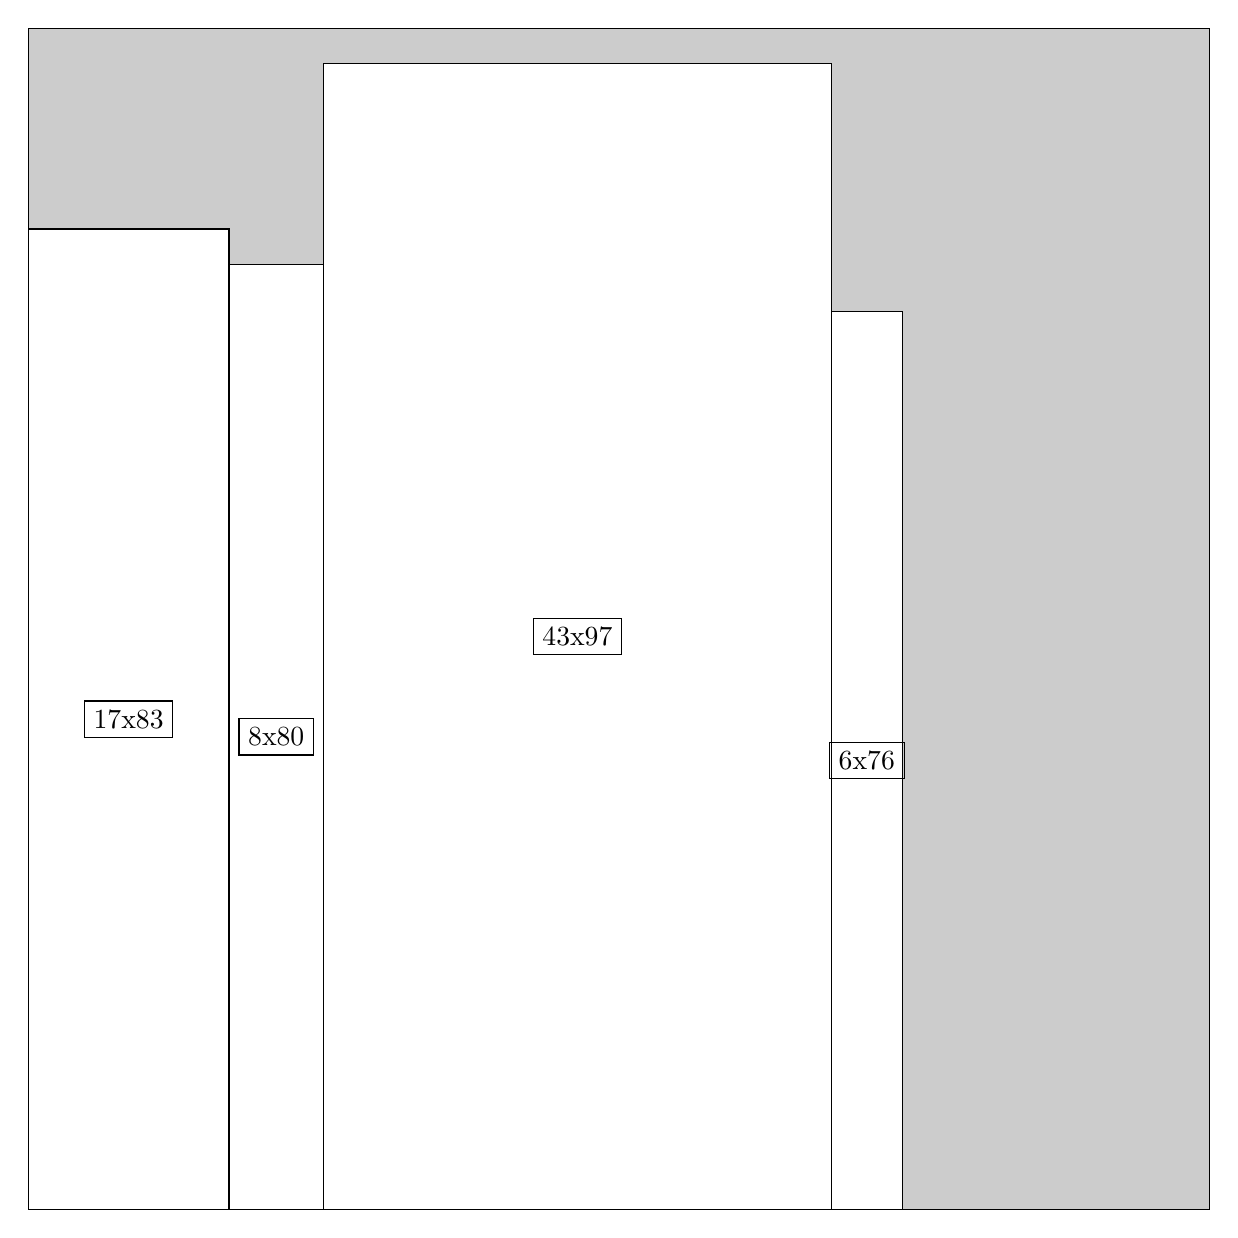
\begin{tikzpicture}[shorten >=1pt,scale=1.0,every node/.style={scale=1.0},->]
\tikzstyle{vertex}=[circle,fill=black!25,minimum size=14pt,inner sep=0pt]
\filldraw[fill=gray!40!white, draw=black] (0,0) rectangle (15.0,15.0);
\foreach \name/\x/\y/\w/\h in {17x83/0.0/0.0/2.55/12.45,8x80/2.55/0.0/1.2/12.0,43x97/3.75/0.0/6.45/14.549999999999999,6x76/10.2/0.0/0.8999999999999999/11.4}
\filldraw[fill=white!40!white, draw=black] (\x,\y) rectangle node[draw] (\name) {\name} ++(\w,\h);
\end{tikzpicture}


w =17 , h =83 , x =0 , y =0 , v =1411
\par
w =8 , h =80 , x =17 , y =0 , v =640
\par
w =43 , h =97 , x =25 , y =0 , v =4171
\par
w =6 , h =76 , x =68 , y =0 , v =456
\par
\newpage


\end{document}